%! Author = Joel Vontobel
%! Date = \today


\documentclass[11pt, a4paper]{report}

% Listings
\usepackage{listings}

\lstset{
    literate={ö}{{\"o}}1
        {ä}{{\"a}}1
        {ü}{{\"u}}1
}

\lstset{language=Java,
    basicstyle=\ttfamily,
    keywordstyle=\color{javapurple}\bfseries,
    stringstyle=\color{javared},
    commentstyle=\color{javagreen},
    morecomment=[s][\color{javadocblue}]{/**}{*/},
    numbers=left,
    numberstyle=\tiny\color{black},
    stepnumber=2,
    numbersep=10pt,
    tabsize=4,
    showspaces=false,
    showstringspaces=false}

% Packages
\usepackage[margin=1.4in]{geometry}
\usepackage[T1]{fontenc}
\usepackage[utf8]{inputenc}
\usepackage[ngerman]{babel}
\usepackage{hyperref}
\usepackage{verbatim}
\usepackage{graphicx}
\usepackage{float}
\usepackage{pdfpages}
\usepackage[
    singlelinecheck=false
]{caption}
\usepackage[raggedright]{titlesec}
\usepackage[nottoc]{tocbibind}
\usepackage{longtable}
\usepackage{tocloft}
\usepackage{fancyhdr}
\usepackage{lastpage}
\usepackage{pifont}
\usepackage{amsmath}

\usepackage[automake]{glossaries-extra}
\usepackage{wasysym}
\usepackage{textcomp}
\usepackage{color}



\titleformat{\chapter}{\normalfont\bfseries\LARGE\raggedright}{\thechapter}{1ex}{}
\titlespacing*{\chapter}{0pt}{30pt}{30pt}
\setcounter{secnumdepth}{3}
\setcounter{tocdepth}{3}
\setlength{\cftsecnumwidth}{2.8em}
\renewcommand\labelitemi{$-$}
\renewcommand\labelitemii{$-$}
\renewcommand\labelitemiii{$-$}
\renewcommand{\headrulewidth}{0pt}

\usepackage[
    backend=biber,
    citestyle=authoryear,
    style=authoryear,
]{biblatex}
\addbibresource{global/quellen.bib}

\usepackage[toc]{glossaries}
\makeglossaries
\loadglsentries{global/glossar_eintraege}

\pagestyle{fancy}
\fancyhf{}
\renewcommand{\headrulewidth}{0pt}
%TODO Platzhalter ersetzen
\lfoot{\fontsize{10}{15} \selectfont Joel Vontobel}
\cfoot{\fontsize{10}{15} \selectfont \today}
\rfoot{\fontsize{10}{15} \selectfont \thepage~von~\pageref*{LastPage}}
\fancypagestyle{plain}{}

\newcommand{\oksymbol}{{\color{green}\ding{51}}}
\newcommand{\errorsymbol}{{\color{red}\ding{55}}}

\makeatletter
\def\blx@citation#1#2{\blx@citation@entry{#1}{#2}}
\makeatother
\renewcommand{\arraystretch}{1.5}
% Document
\begin{document}

    \begin{titlepage}

    \begin{figure}
        \begin{center}
            
\includegraphics[width=0.6\textwidth]{ressourcen/ergon_logo_gross}
            \captionsetup{textformat=empty, labelformat=empty}
            \caption[Logo der Ergon Informatik AG~\parencite{ergonlogo}]{Logo der Ergon Informatik AG}\label{fig:ergon-logo-gross}
        \end{center}
    \end{figure}
    \begin{center}
        \vspace*{2cm}
        \Huge
        \textbf{Probe-IPA}

        \vspace{0.5cm}
        \Large
        %TODO Platzhalter ersetzen 
        Eingehende Message-Queue-Nachrichten im Web-UI

        \vfill

        \Large
        %TODO Platzhalter ersetzen
        Probe-IPA von Joel Vontobel

        \vspace*{3cm}

        \large
        Ergon Informatik AG\\
        \today\\

    \end{center}
\end{titlepage}

    \renewcommand*\contentsname{Inhalt}
\tableofcontents
    \part{Umfeld und Ablauf}\label{part:1}

    \chapter{Aufgabenstellung}\label{ch:aufgabenstellung}
In diesem Kapitel ist die Aufgabenstellung der Probe-IPA aufgeführt. Die Inhalte wurden zu einem grossen Teil von der originalen Aufgabenstellung übernommen und Angepasst.

\section{Ausgangslage}\label{sec:ausgangslage}
Die Firma \gls{Ergon Informatik AG} entwickelt sein einigen Jahren eine Transaktions-Authorisierungs-Lösung für einige Banken in der Schweiz. Dieses Projekt heisst \gls{CardX} und wird durch ein 12 zwölfköpfiges Team umgesetzt. In diesem Projekt ist der Lernende seit Januar 2024 tätig und kennt sich deshalb schon ein bisschen aus.

Das Projekt kommuniziert mit verschiedenen bankspeziefischen IT-Systemen wie zum Beispiel dem Kernbankensystem oder Service-Büros über Message-Queues. Diese Message-Queues werden in der Datenbank-Tabelle MQ\_TABLE (eingehende Nachrichten) und MQ\_OUT (ausgehende Nachrichten) zwischengespeichert. Falls man diese Message-Queues anschauen oder bearbeiten möchte, muss man dies in der Datenbank machen. Weil das ziemlich umständlich ist, besteht die Aufgabe des Lernenden jetzt daraus diese Message-Queues in einem \gls{Web-GUI} darzustellen und sinnvolle Interaktionen mit diesen Daten anzubieten.

\section{Detaillierte Aufgabenstellung}\label{sec:detaillierte-aufgabenstellung}

\paragraph{Minimalanforderungen}
Das Ziel dieser Aufgabe ist es, den Inhalt der Tabelle MQ\_TABLE in diesem Web-GUI sichtbar zu machen und dem Nutzer sinnvolle Interaktionen mit diesen Daten anzubieten.

Es soll im Weg-GUI eine neue Seite erstellt werden mit dem Inhalt einer Tabelle, welche die Message-Queues abbilden soll. Die Tabelle soll eine Hand voll Spalten besitzen, sodass sie übersichtlicher ist. Die Seite soll stimmig in das \gls{UI} eingebaut werden. Im \gls{Backend} sollen die neuen Methoden mithilfe von Unit-Tests abgedeckt werden.

Zusätzlich kann der Lernende noch zwischen zwei Erweiterungen entscheiden, welche er implementieren möchte.

\paragraph{Erweiterung: Pagination}
Bei der ersten Erweiterungen ist das Ziel ein Paginator zur Tabelle hinzuzufügen. Eine Pagination ist wenn man eine Liste oder Tabelle auf ein paar Einträge limitiert und anschliessend weitere Einträge anzeigen kann mit einer Pfeiltaste. Dies hilft, das Laden der Seite zu verkürzen, da die Einträge, die nicht angezeigt werden, erst geladen werden, wenn sie auch wirklich gebraucht werden.

\paragraph{Erweiterung: Filter}
Die zweite Erweiterung ist ein Filtersystem. Die Seite soll nach dem Status, Inhalt der Nachricht und dem Datum gefiltert werden können. Die Filter-Werte sollen ausserdem in der URL Abgebildet werden, um das Teilen von gefilterten Ergebnissen zu vereinfachen oder den Filter als Lesezeichen abgelegen zu können.

\section{Mittel und Methoden}\label{sec:mittel-und-methoden}

\paragraph{Technologien}
\begin{itemize}
	\item SQL
    \item Java
    \item TypeScript
    \item HTML
    \item Angular
\end{itemize}

\paragraph{Tools}
\begin{itemize}
	\item IntelliJ (IDE)
    \item Docker
	\item Bitbucket
	\item Confluence
	\item Jira
	\item Postman
\end{itemize}

\section{Vorkenntnisse}\label{sec:vorkenntnisse}
Der Lernende hat bereits viele Arbeiten im Projekt CardX gemacht. Unter anderem im Backend und an CardX-spezifischen Tools. Die Codebasis hat der Lernende in den letzten 9 Monaten gut kennengelernt und findet sich gut zurecht. Der Lernende hat auch bereits die Tabelle TASK von der Datenbank in das Web-GUI gebracht, was eine ähnliche Aufgabe war wie die jetzige Aufgabenstellung.

Durch die früheren Projekte, wie ein Fussballtippspiel und eine Anmelde-Plattform für Bewerbende, konnte er bereits viel Erfahrung mit Java und Angular sammeln.

\section{Vorarbeiten}\label{sec:vorarbeiten}
Durch das bereits existierende Projekt und die vielen Arbeiten, die der Lernende bereits gemacht hat, musste er keine Vorarbeiten leisten.

\section{Neue Lerninhalte}\label{sec:neue-lerninhalte}
\begin{itemize}
    \item Pagination: 
    
    Mit Pagination hat der Lernende sich noch nie auseinandergesetzt. Er hat es schon oft auf anderen Seiten gesehen aber noch nie selbst implementiert.
    \item Filtersystem:
    
    Im Projekt WM-Tippspiel gab es ein Filtersystem, aber dieses hat der Lernende nicht selbst implementiert und ist so ein neuer Lerninhalt.
\end{itemize}

\section{Arbeiten in den letzten 6 Monaten}\label{sec:arbeiten-in-den-letzten-6-monaten}
In den letzten 6 Monaten hat der Lernende sich, wie oben schon genannt, mit dem Projekt CardX auseinandergesetzt und ist ein aktives Team Mitglied. Er hat viele verschiedene Arbeiten umgesetzt. Einige davon hier:
\begin{itemize}
    \item CheckDB Task:
    
    In dieser Aufgabe geht es darum, eine Aufgabe zu erstellen, welche periodisch oder manuell ausgeführt werden kann. Diese Aufgabe überprüft die Datenbankdefinition, ob immer noch alles fehlerfrei ist. Es werden Sequenzen, Indexe, Felder und mehr in eine Datei geschrieben, gespeichert und anschliessend mit der vorherigen Datei auf Veränderungen verglichen. Bei einer Veränderung schlägt die Aufgabe fehl und die Differenz wird in der Fehlermeldung angezeigt.
    \item ServiceLogMove und Zip:
    
    Mit der Aufgabe ServiceLogMerge werden Protokolle des Systems in Dateien geschrieben und gespeichert. Ein Teil dieser Dateien wird jetzt mithilfe der Aufgabe in bestimmte Verzeichnisse verschoben und komprimiert. Die Dateien werden nach Bank sortiert und anschliessend in ihn vorgesehenes Verzeichnis verschoben. Auch diese Aufgabe wird periodisch jeden Tag ausgeführt, um die Dateiablage übersichtlich zu halten.
    \item Tasks im Frontend anzeigen und bearbeiten:
    
    Diese Aufgabe zeigt alle Tasks im Frontend an und man kann sie dort auch bearbeiten. Das Ziel von dieser Aufgabe war gleich wie die Mindestanforderungen von der Aufgabenstellung.
    \begin{figure}[H]
    	\begin{center}
    		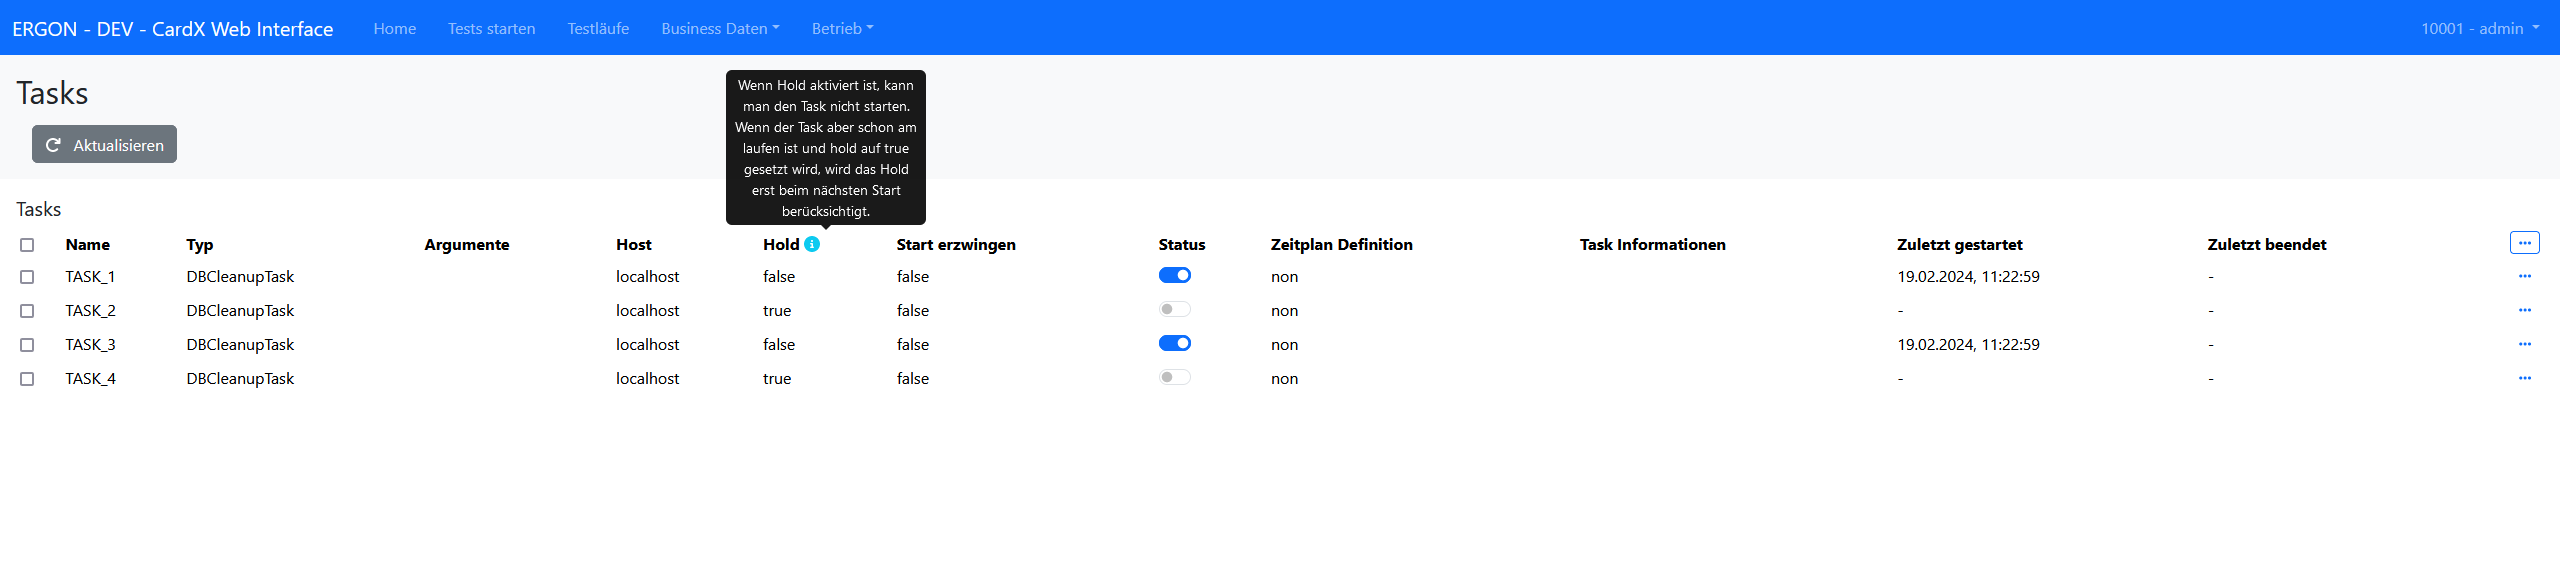
\includegraphics[width=1\textwidth]{ressourcen/show-and-edit-tasks}
    		\caption[Anzeigen und bearbeiten der Tasks]{Anzeigen und bearbeiten der Tasks}\label{fig:show-and-edit-tasks}
    	\end{center}
    \end{figure}
\end{itemize}

    \chapter{Projektaufbauorganisation}\label{ch:projektaufbauorganisation}
In der folgenden Tabelle sind die an der Probe-IPA beteiligten Personen und ihre jeweiligen Aufgaben aufgeführt.

\renewcommand{\arraystretch}{1.5}
\begin{longtable}{|p{.30\textwidth}|p{.30\textwidth}|p{.40\textwidth}|}
    \hline
    \textbf{Person} & \textbf{Rolle} & \textbf{Aufgabe/Verantwortung} \\
    \hline
    %TODO Platzhalter ersetzen
    \hypertarget{k}{Joel Vontobel} & Kandidat (K) & Umsetzen der Facharbeit \\
    \hline
    %TODO Platzhalter ersetzen
    \hypertarget{vf}{Loris Diana und Dominic Monzón} & Verantwortliche Fachkraft (VF) & Facharbeit begleiten, technische Fragen beantworten, Bewertung der Facharbeit \\
    \hline
    %TODO Platzhalter ersetzen
    \hypertarget{hex}{Bernd Lienberger} & Hauptexperte (HEX) & IPA bezogene Fragen beantworten, Entscheiden bei auftretenden Problemen, Besuchstermine festlegen, Fachgespräch leiten, Bewertung der Facharbeit \\
    \hline
    %TODO Platzhalter ersetzen
    \hypertarget{nex}{} & Nebenexperte (NEX) & Notizen erstellen zu Präsentation und zum Fachgespräch, Bewertung der Facharbeit \\
    \hline
\end{longtable}
\renewcommand{\arraystretch}{1}

    \chapter{Benützte Firmenstandards}\label{ch:benuetzte-firmenstandards}
Es werden keine spezifischen Firmenstandards verwendet.

    \chapter{Arbeitsumgebung}\label{ch:arbeitsumgebung}
In diesem Kapitel ist beschrieben, wie die Arbeitsumgebung des Lernenden während der Probe-IPA aussah.


\section{Arbeitsplatz}\label{sec:arbeitsplatz}
\subsection{Office Arbeitsplatz}\label{subsec:office-arbeitsplatz}
Die Probe-IPA wird am gewohnten Arbeitsplatz im Fünferbüro des Lernenden durchgeführt. Als Arbeitsgerät wird ein Notebook verwendet, welches mithilfe einer Dockingstation das Gerät mit zwei Monitoren und dem Firmennetzwerk verbindet. Der Stuhl und Tisch sind höhenverstellbar, und der Lernende kann dadurch in verschiedenen Sitzpositionen oder stehend arbeiten.

\begin{figure}[H]
    \begin{center}
        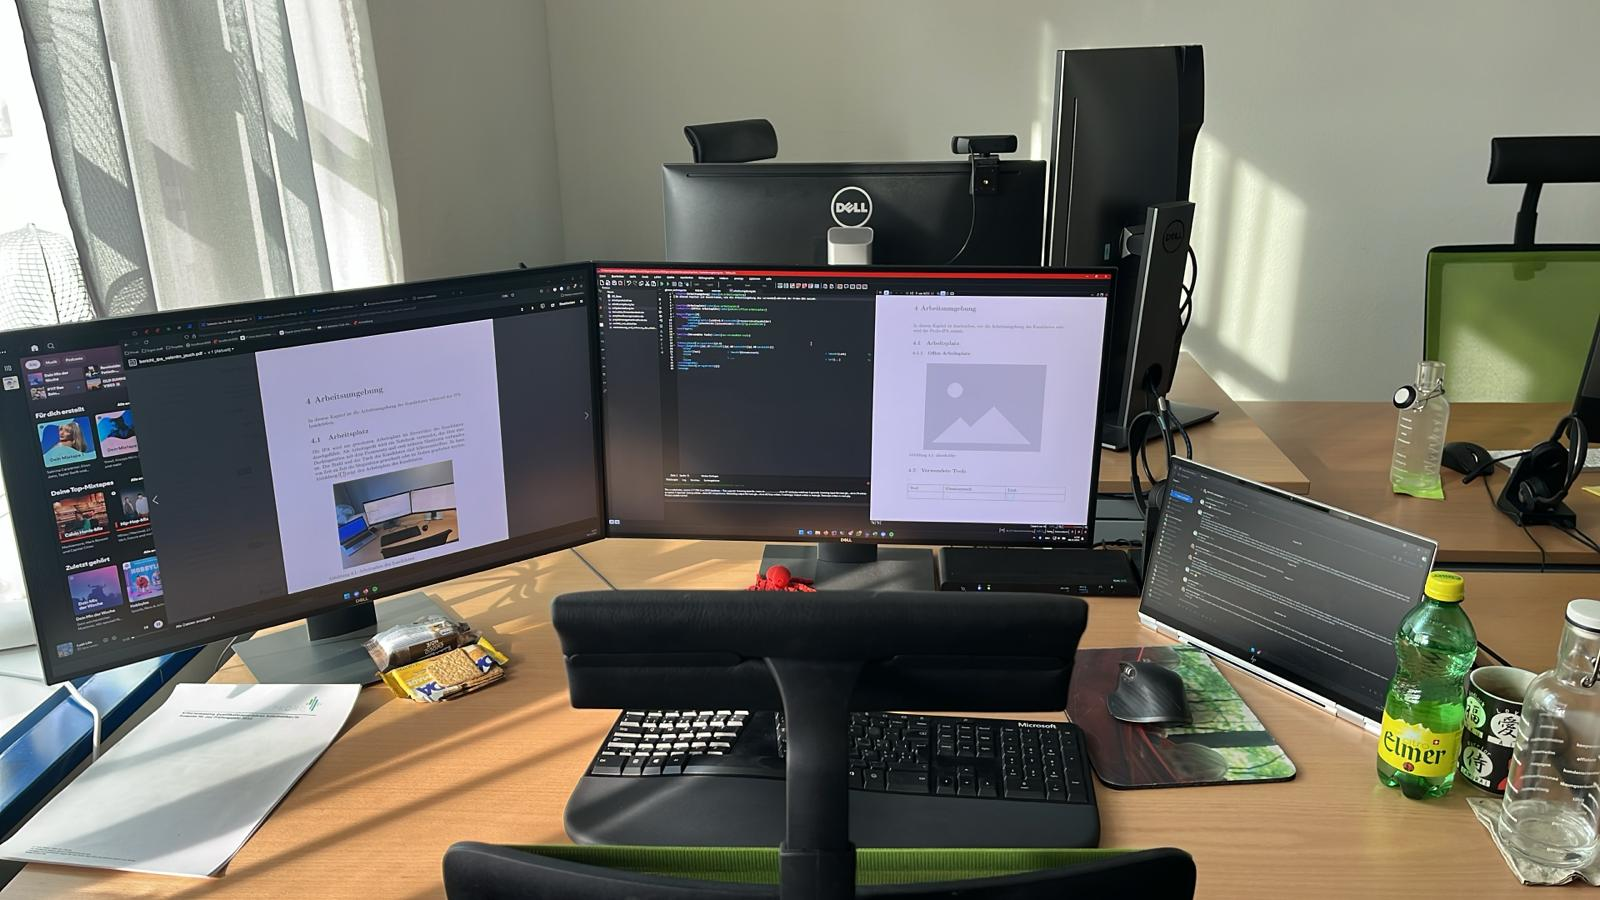
\includegraphics[width=0.8\textwidth]{ressourcen/Arbeitsplatz-Joel-Vontobel}
        \caption[Arbeitsplatz des Lernenden]{Arbeitsplatz des Lernenden}\label{fig:Arbeitsplatz-Joel-Vontobel}
    \end{center}
\end{figure}

\newpage
\section{Verwendete Tools}\label{sec:verwendete-tools}
Die folgende Tabelle zeigt auf, welche Tools für die Umsetzung der Probe-IPA eingesetzt wurden.

\renewcommand{\arraystretch}{1.5}
\begin{longtable}{|p{.22\textwidth}|p{.40\textwidth}|p{.38\textwidth}|}
    \hline
    \textbf{Tool}                    & \textbf{Einsatzzweck}                              & \textbf{Link}                                                             \\ \hline
    IntelliJ                         & Entwicklungsumgebung für die Programmierung        & \url{https://www.jetbrains.com/de-de/idea/}                               \\ \hline
    Docker                           & Ausführen der Programme                            & \url{https://www.docker.com/}                                             \\ \hline
    Git                              & Versionierung vom Quellcode                        & \url{https://git-scm.com/}                                                \\ \hline
    Postman                          & Ausführen von HTTP-Requests (Testen vom Bankend)   & \url{https://www.postman.com/}                                            \\ \hline
    Bitbucket                        & Speicherung der Quellcodes                         & \url{https://bitbucket.org/product/}                                      \\ \hline
    Confluence                       & Probe-IPA Kriterien                                & \url{https://www.atlassian.com/de/software/confluence}                    \\ \hline
    Jira                             & Aufgabenstellung                                   & \url{https://www.atlassian.com/de/software/jira}                          \\ \hline
    Draw.io                          & Erstellen von Diagrammen und Abbildungen           & \url{https://www.drawio.com/}                                             \\ \hline
    TexStudio                        & Dokumentationstool                                 & \url{https://www.texstudio.org/}                                          \\ \hline
    LaTeX                            & Ein Dokumentenvorbereitungssystem                  & \url{https://www.latex-project.org/}                                      \\ \hline
    Mattermost                       & Text basiertes Kommunikationsmittel                & \url{https://mattermost.com/}                                             \\ \hline
    Microsoft Teams                  & Video basiertes Kommunikationiesmittel             & \url{https://www.microsoft.com/de-ch/microsoft-teams/group-chat-software} \\ \hline
    Microsoft Excel                  & Erstellung und Bearbeitung des Zeitplans           & \url{https://www.microsoft.com/de-ch/microsoft-365/excel?market=ch}       \\ \hline
\end{longtable}
\renewcommand{\arraystretch}{1}
\newpage
    \chapter{Versionierung und Sicherung der Arbeitsergebnisse}\label{ch:versionierung-und-sicherung-der-arbeitsergebnisse}
In diesem Kapitel wird beschrieben, wie der Lernende sicherstellt, dass die erarbeiteten Ergebnisse während der Probe-IPA sicher gespeichert und jederzeit wieder aufrufbar sind. Die Versionierung soll es ermöglichen, frühere erstellte Versionen der Daten jederzeit wiederherstellen zu können. Die Massnahmen werden hier vom Lernenden aufgeführt.

\section{Verwendung von Git zu Versionierung}
Für die Versionierung von der Probe-IPA wird Git verwendet. Git ist ein Versionierungstool und wird verwendet, um Quellcode zu versionieren und zu beschriften. In der Schule so wie auch in der Firma wurde Git bereits in diversen Projekten verwendet, um den Quellcode übersichtlich zu versionieren und in der Cloud zu sichern. Mit Git kann man sogenannte «Commits» machen, um einen kleinen Teil der Änderungen zu speichern und zu beschriften. Diese Änderungen kann man jederzeit aufrufen oder wieder rückgängig machen, um eine bestimmte Version genauer zu analysieren. Durch diese Commits ist der Quellcode für eine andere Person verständlicher und einfacher zu lesen.

\section{Quellcode}
Der Quellcode der eingehenden Message-Queue-Nachrichten im Web-GUI wird mit Git verwaltet und ist in einem Repository auf Bitbucket gespeichert. In Abbildung 5.1 ist die Git Commit History des Quellcodes ersichtlich.

\begin{figure}[H]
	\begin{center}
		
\includegraphics[width=0.8\textwidth]{ressourcen/placeholder}
		\caption[Git Commit History des Quellcodes]{Git Commit History des Quellcodes}\label{fig:Git-Commit-History-des-Quellcodes}
	\end{center}
\end{figure}

\section{Probe-IPA Dokumentation}
Die Probe-IPA-Dokumentation wird mithilfe von \LaTeX geschrieben, wodurch eine Versionierung mit Git auch möglich wird. Die \LaTeX- und alle anderen benötigten Dateien werden auf ein privates Repository in der Cloud geladen. In Abbildung 5.2 ist die Git Commit History der Probe-IPA-Dokumentation ersichtlich.

\begin{figure}[H]
	\begin{center}
		
\includegraphics[width=0.8\textwidth]{ressourcen/placeholder}
		\caption[Git Commit History der Dokumentation]{Git Commit History der Dokumentation}\label{fig:Git-Commit-History-der-Dokumentation}
	\end{center}
\end{figure}
    \chapter{Projektmanagementmethode}\label{ch:projektmanagementmethode}
In diesem Kapitel ist die Projektmanagement-Methode «IPERKA» beschrieben, die während der Probe-IPA verwendet wird. Es werden die Gründe für diese Projektmanagement-Methode aufgeführt und eine alternative Methode mit Gründen, warum sie nicht verwendet wurde.

\section{IPERKA}\label{sec:METHODE}
Als Projektmanagement-Methode während der Probe-IPA wird IPERKA verendet. IPERKA ist eine Vorgehensmethode, die sich gut für Projekte mit überschaubarem Umfang und klar definierte Ziele eignet. Die Methode wirde bereits im ersten Lehrjahr in der Schule behandelt und ist durch das bereits bekannt. Der Name «IPERKA» setzt sich aus den Anfangsbuchstaben der sechs verschiedenen Schritten zusammen, nach denen vorgegangen wird:

\paragraph{I} nformieren: Den Auftrag verstehen, eine Vorstellung der Lösung erhalten, fehlende Informationen einholen, ordnen und bewerten
\paragraph{P} lanen: Nötige Arbeitsschritte definieren, einen Zeitplan erstellen, Methoden und Arbeitsmittel definieren
\paragraph{E} ntscheiden: Verschiedene Lösungsvarianten vergleichen, ausschlaggebende Kriterien definieren, eine Lösungsvariante auswählen
\paragraph{R} ealisieren: Arbeit umsetzen, Arbeitsschritte und Ergebnisse dokumentieren, auftrettende Probleme behandeln
\paragraph{K} ontrollieren: Arbeit testen, Resultate mit den Anforderungen vergleichen, Soll-Ist-Vergleich des Zeitplans, Dokumentation nochmals durchlesen
\paragraph{A} uswerten: Rückblick auf das Vorgehen, Arbeitsschritte beurteilen, Selbsteinschätzung vornehmen, mögliche Optimierungen für weitere Projekte definieren

\pagebreak
Die Aufteilung der Arbeit in die genannten Schritte unterstützt dabei, die Aufgaben sinnvoll zu strukturieren und systematisch vorzugehen. Ausserdem hilft die bewusste Steuerung des Arbeitsprozesses, die persönlichen Kompetenzen weiterzuentwickeln (vgl. ICT Berufsbildung Bern 2024\parencite{ict}). Die klare Trennung der Schritte stellt sicher, dass der Umfang und die erwarteten Ergebnisse der Aufgabe sich im Verlauf der Arbeit nicht mehr stark ändern, da IPERKA grundsätzlich kein «Rückwärtsgehen» in den Phasen, wie dies aus iterativen Modellen bekannt ist, vorsieht. Ausserdem stellt sie sicher, dass die Realisierung nicht zu schnell in Angriff genommen wird.

\section{Alternative Methode}\label{sec:alternative-methode}
Neben IPERKA wurde noch eine andere Vorgehensmethode angeschaut. Diese ist folgend, jeweils mit einer Begründung, wieso IPERKA der Methode vorgezogen wurde, kurz beschrieben.

\paragraph{Scrum} ist eine bekannte agile Vorgehensmehtode, die heutzutage in der Softwareentwicklung weit verbreitet ist. Die Methode legt den Fokus mehr auf Punkte wie laufende Software, gute Zusammenarbeit, oder flexibles Reagieren auf Veränderungen, ansttt einem strikten Plan zu folgen. Scrum sieht einen iterativen Prozess vor, der laufend optimiert werden soll, und definiert verschiedene Rollen, die jeweils ihre Aufgabe in diesem Scrum-Prozess haben. Ein «agiles» Vorgehen ist in der Softwareentwicklung grundsätzlich sinnvoll, da oft nicht von Beginn her klar ist, wie das Resultat schlussendlich aussehen soll. Da die Probe-IPA schlussendlich aber eine Prüfung ist, sind die Vorgaben und erwarteten Resultate relativ klar. Auch der Umfang der Probe-IPA und das Enddatum sind von Beginn an bekannt und verändern sich nicht während der Arbeit. Ausserdem wird die Aufgabe von nur einer Person bearbeitet, wofür die Abläufe von Scrum nicht optimal geeignet sind. Aus diesen Gründen wird IPERKA gegenüber Scrum vom Lernenden bevorzugt.

    \chapter{Arbeitsprotokoll}\label{ch:arbeitsprotokoll}
\renewcommand{\arraystretch}{1.5}

\begin{longtable}{p{.22\textwidth}|p{.78\textwidth}}
	\hline
	\textbf{Datum}                       & 06.11.2024            \\
	\hline
	\textbf{Bearbeitete Arbeitspakete}   & 7.1, 7.2, 7.3, 7.4                  \\
	\hline
	\textbf{Arbeitszeit}                 & 8h                                    \\
	\hline
	\textbf{Überzeit}                    & 0h                                    \\
	\hline
	\textbf{Vergleich mit dem Zeitplan}  & Zeitplan noch nicht fertig \\
	\hline
	\textbf{Erfolge und Probleme} & Durch die Vorlage des Dokuments und \LaTeX konnte ich direkt mit dem ersten Teil der Dokumentation beginnen, was mir viel Zeit erspart hat. Ich habe heute mein Ziel, den ersten Teil grösstenteils abzuschliessen, erreicht und hatte keine grösseren Probleme, die aufgetreten sind.
	\\
	\hline
	\textbf{Tagesreflexion} & Ich bin heute gut in die Probe-IPA gestartet. Anfangs war ich ein wenig überfordert und wusste nicht, wo ich anfangen sollte. Nach der ersten Stunde hat sich das aber wieder gelegt und ich konnte konzentriert an meinem Ziel arbeiten.
	\\
	\hline
	\textbf{In Anspruch genommene Hilfe} & Keine                              \\
	\hline
\end{longtable}\label{tab:arbeitsprotokoll-06.11.2024}
\newpage

\begin{longtable}{p{.22\textwidth}|p{.78\textwidth}}
	\hline
	\textbf{Datum}                       & 07.11.2024            \\
	\hline
	\textbf{Bearbeitete Arbeitspakete}   & 1.1, 1.2, 2.1, 2.2                  \\
	\hline
	\textbf{Arbeitszeit}                 & 8h                                    \\
	\hline
	\textbf{Überzeit}                    & 0h                                    \\
	\hline
	\textbf{Vergleich mit dem Zeitplan}  & Ich konnte alle geplanten Arbeiten von heute erledigen und hatte auch eine Stunde übrig. Ich habe also bereits mit der Aufgabe 2.3 angefangen. \\
	\hline
	\textbf{Erfolge und Probleme} & Heute konnte ich mit dem 2. Teil der Dokumentation anfangen. Die Phase Informieren konnte ich zeitgerecht abschliessen und habe bereits in der Phase Planen die Arbeitspakete und den Zeitplan fertiggestellt. Momentan habe ich mit der Aufgabe \ref{tab:planen-2.3} begonnen, die für morgen eingeplant ist.
	\\
	\hline
	\textbf{Tagesreflexion} & Ich konnte heute motiviert in den Tag starten, da ich gestern meine Tagesziele erreicht habe. Ich konnte mich nicht wirklich für \ref{tab:informieren-1.1} und \ref{tab:informieren-1.2} motivieren, wusste aber, dass ich mich danach mit den Arbeitspaketen und dem Zeitplan beschäftigen kann. Diese zwei Teile haben mir Spass gemacht, da ich mich danach am Zeitplan orientieren kann.
	\\
	\hline
	\textbf{In Anspruch genommene Hilfe} & Ich habe mich bei Loris Diana \ref{ch:projektaufbauorganisation} erkundigt, ob ich die Codequalität mit dem Tool, welches mein Projekt nutzt, überprüfen darf oder ich selbst diese Überprüfung machen muss.                                \\
	\hline
\end{longtable}\label{tab:arbeitsprotokoll-07.11.2024}
\newpage

\begin{longtable}{p{.22\textwidth}|p{.78\textwidth}}
	\hline
	\textbf{Datum}                       & 08.11.2024            \\
	\hline
	\textbf{Bearbeitete Arbeitspakete}   & 2.3, 2.4                  \\
	\hline
	\textbf{Arbeitszeit}                 & 8h                                    \\
	\hline
	\textbf{Überzeit}                    & 0h                                    \\
	\hline
	\textbf{Vergleich mit dem Zeitplan}  & Ich konnte alle geplanten Arbeitspakete machen oder anfangen.  \\
	\hline
	\textbf{Erfolge und Probleme} & Heute hatte ich Probleme mit der Konzentration. Sie ist schwungartig gekommen und wieder gegangen. Durch das habe ich ein wenig Zeit verloren und bin jetzt wieder im Zeitplan. Mein Ziel für heute war eigentlich, das Arbeitspaket 2.5 fertig zu haben, sodass ich nächste Woche mit dem Testkonzept starten kann. Ich habe es nicht ganz geschafft. Es fehlt aber nicht mehr viel.
	\\
	\hline
	\textbf{Tagesreflexion} & Wie bei «Erfolge und Probleme» schon erwähnt, fehlte mir heute ein wenig die Konzentration. Ich glaube, es könnte mit der VA zusammenhängen, da ich diese Woche noch daran gearbeitet habe und ich so mehrheitlich am Schreiben war. Ansonsten kann ich mich nicht beklagen, da ich immer noch ein kleines bisschen im Vorsprung zum Zeitplan bin.
	\\
	\hline
	\textbf{In Anspruch genommene Hilfe} & Ich habe mich heute bei Dominic Monzón \ref{ch:projektaufbauorganisation} erkundigt, ob für die Filterung alle MQ\_IN\_STATI gebraucht werden, weil im Quellcode die einen mit «// TODO huberdav: can be removed eventually» beschriftet sind.                                \\
	\hline
\end{longtable}\label{tab:arbeitsprotokoll-08.11.2024}
\newpage

\begin{longtable}{p{.22\textwidth}|p{.78\textwidth}}
	\hline
	\textbf{Datum}                       & 12.11.2024            \\
	\hline
	\textbf{Bearbeitete Arbeitspakete}   & 2.5                  \\
	\hline
	\textbf{Arbeitszeit}                 & 3.5h                                    \\
	\hline
	\textbf{Überzeit}                    & -0.5h                                    \\
	\hline
	\textbf{Vergleich mit dem Zeitplan}  & Momentan bin ich auf Kurs mit dem Zeitplan und habe keine Abweichungen. \\
	\hline
	\textbf{Erfolge und Probleme} & Alle Lösungskonzepte sind fertig und ich konnte mit den Testkonzepten anfangen.
	\\
	\hline
	\textbf{Tagesreflexion} & Heute kam ich gut voran und bin immer noch im Zeitplan. Der Vorsprung von letzter Woche ist heute jedoch nicht mehr vorhanden, aber ich bin nicht im Verzug. Heute war die Konzentration wieder hoch und ich hoffe, das bleibt auch für die bleibenden Tage noch weiter so.
	\\
	\hline
	\textbf{In Anspruch genommene Hilfe} & Ich habe mich bei Loris Diana \ref{ch:projektaufbauorganisation} erkundigt, ob ein Integration-Test für einen Endpoint eine Datenbank braucht, die läuft. Er hat mir erklärt, dass es eine braucht, aber auch eine In-Memory-Datenbank ausreicht.                              \\
	\hline
\end{longtable}\label{tab:arbeitsprotokoll-12.11.2024}
\newpage

\begin{longtable}{p{.22\textwidth}|p{.78\textwidth}}
	\hline
	\textbf{Datum}                       & 13.11.2024            \\
	\hline
	\textbf{Bearbeitete Arbeitspakete}   & 2.6, 3.1, 4.1                  \\
	\hline
	\textbf{Arbeitszeit}                 & 8.5h                                    \\
	\hline
	\textbf{Überzeit}                    & 0.5h                                    \\
	\hline
	\textbf{Vergleich mit dem Zeitplan}  & Durch die nicht verwendeten 3 Stunden von der Entscheidung wurde ich heute bei dem Punkt 4.1 zwei Stunden früher als geplant fertig. \\
	\hline
	\textbf{Erfolge und Probleme} & Heute konnte ich nach vielen Tagen Dokumentation schreiben, endlich mit dem Programmieren anfangen. Ich habe den Endpunkt bereits fertig und Dokumentiere diesen jetzt.
	\\
	\hline
	\textbf{Tagesreflexion} & Mit viel Motivation startete ich heute in den Tag, da ich wusste, dass ich endlich mit dem Programmieren anfangen kann. Ich habe das Textkonzept fertig geschrieben und konnte ziemlich schnell die Entscheidung abschliessen und habe so zwei Meilensteine in meiner Probe-IPA erreicht.
	\\
	\hline
	\textbf{In Anspruch genommene Hilfe} & Ich hatte Probleme mit einem Bean in Java, welches für den MqInService gebraucht wurde. Dieses wurde nicht gefunden und Dominic Monzón \ref{ch:projektaufbauorganisation} hat mir geholfen, dieses für den Service zu erstellen. Ausserdem konnte ich den Endpoint nicht ansprechen, da die Url fälschlicherweise falsch war und habe mir Hilfe von Micha Schena geholt (Ein Mitarbeiter im CardX-Team).                              \\
	\hline
\end{longtable}\label{tab:arbeitsprotokoll-13.11.2024}
\newpage

\begin{longtable}{p{.22\textwidth}|p{.78\textwidth}}
	\hline
	\textbf{Datum}                       & 14.11.2024            \\
	\hline
	\textbf{Bearbeitete Arbeitspakete}   & 4.2                  \\
	\hline
	\textbf{Arbeitszeit}                 & 8h                                    \\
	\hline
	\textbf{Überzeit}                    & 0h                                    \\
	\hline
	\textbf{Vergleich mit dem Zeitplan}  & Momentan bin ich synchron mit dem Zeitplan. \\
	\hline
	\textbf{Erfolge und Probleme} & Heute konnte ich die Mindestanforderungen abschliessen und mit der Erweiterung weiter machen.
	\\
	\hline
	\textbf{Tagesreflexion} & Ich konnte heute wieder mit viel Motivation in den Tag starten, da heute die Implementierung im Frontend bevor stand. Ich hatte länger als gedacht, da ich gestern einen Endpoint vergessen habe zu implementieren, welcher ich heute nacharbeiten musste.
	\\
	\hline
	\textbf{In Anspruch genommene Hilfe} & Loris Diana \ref{ch:projektaufbauorganisation} hat mir heute erklärt, wie die Generierung von den HTTP-Requests im Frontend genau funktioniert.                              \\
	\hline
\end{longtable}\label{tab:arbeitsprotokoll-14.11.2024}
\newpage

\begin{longtable}{p{.22\textwidth}|p{.78\textwidth}}
	\hline
	\textbf{Datum}                       & 15.11.2024            \\
	\hline
	\textbf{Bearbeitete Arbeitspakete}   & 4.3, 4.5                  \\
	\hline
	\textbf{Arbeitszeit}                 & 8h                                    \\
	\hline
	\textbf{Überzeit}                    & 0h                                    \\
	\hline
	\textbf{Vergleich mit dem Zeitplan}  & Da ich die Implementation von 4.4 \ref{tab:realisieren-4.4} pausiert habe, bin ich wieder synchron mit dem Zeitplan. \\
	\hline
	\textbf{Erfolge und Probleme} & Heute hatte ich viele Schwierigkeiten mit der Implementierung der Erweiterung im Frontend. Trotz des Beispiels von «Fehlgeschlagene Zahlung», schaffte ich es nicht, ein Filterergebnis im Frontend anzeigen zu lassen. Ich habe vieles ausprobiert und werde, falls noch Zeit ist, mit einem Fachverantwortlichen das Problem nochmals angehen.
	\\
	\hline
	\textbf{Tagesreflexion} & Ich hatte heute viel Motivation, um die Implementierung für den grössten Teil zu ermöglichen. Leider schwand diese Motivation ziemlich schnell während der Implementierung der Erweiterung im Frontend. Anfangs kam ich noch gut voran. Mit der Zeit wusste ich aber nicht, ob diese Implementierung funktionieren wird oder nicht. Da ich für beide Implementationen (das Backend und Frontend der Erweiterung) noch keine Dokumentation geschrieben habe, habe ich mich dazu entschieden, die Implementation zu pausieren und damit anzufangen, sodass ich nicht noch mehr in den Verzug komme.
	\\
	\hline
	\textbf{In Anspruch genommene Hilfe} & Dominic Moncón \ref{ch:projektaufbauorganisation} hat mir heute eine Frage bezüglich der Filterung beantwortet. Für die Filterung von Nachrichten konnte ich nicht auf die entsprechende Spalte zugreifen, und die Frage war, wie ich jetzt auf sie zugreifen kann. Bei anderen Feldern gibt es eine Variable, welche dies ermöglicht. Oberhalb der Felder steht aber, dass sie generiert wurden, und ich wusste nicht, ob ich sie direkt in dieser Klasse hinzufügen kann oder ob ich anderswo eine kleine Änderung unternehmen muss. Ich konnte schlussendlich einfach diese Variable hinzufügen.                           \\
	\hline
\end{longtable}\label{tab:arbeitsprotokoll-15.11.2024}
\newpage

\begin{longtable}{p{.22\textwidth}|p{.78\textwidth}}
	\hline
	\textbf{Datum}                       & 19.11.2024            \\
	\hline
	\textbf{Bearbeitete Arbeitspakete}   & 5.1 (angefangen)                  \\
	\hline
	\textbf{Arbeitszeit}                 & 3h                                    \\
	\hline
	\textbf{Überzeit}                    & -1h                                    \\
	\hline
	\textbf{Vergleich mit dem Zeitplan}  & Im Moment bin ich noch im Zeitplan. \\
	\hline
	\textbf{Erfolge und Probleme} & Heute konnte ich die Phase Realisieren abschliessen und mit der Implementierung der Tests anfangen. 
	\\
	\hline
	\textbf{Tagesreflexion} & Ich habe heute noch die Mock Implementation vom MqInService gemacht für das Akzeptanzkriterium. Dies ging ziemlich schnell und war nicht schwer zu implementieren. Ausserdem habe ich den ersten Test heute geschrieben, ohne grosse Probleme. Momentan kommen aber die hinzugefügten Daten in der Datenbank noch nicht im Test an. Dieses Problem werde ich aber morgen in Angriff nehmen. 
	\\
	\hline
	\textbf{In Anspruch genommene Hilfe} & -                              \\
	\hline
\end{longtable}\label{tab:arbeitsprotokoll-19.11.2024}
\newpage

\begin{longtable}{p{.22\textwidth}|p{.78\textwidth}}
	\hline
	\textbf{Datum}                       & 20.11.2024            \\
	\hline
	\textbf{Bearbeitete Arbeitspakete}   & 5.1, 5.2 (angefangen), 7.4                  \\
	\hline
	\textbf{Arbeitszeit}                 & 9h                                    \\
	\hline
	\textbf{Überzeit}                    & 1h                                    \\
	\hline
	\textbf{Vergleich mit dem Zeitplan}  & Durch die Verzögerung mit der Prüfung der Codequalität bin ich momentan 4 Stunden im Verzug.\\
	\hline
	\textbf{Erfolge und Probleme} & Heute konnte ich das Schreiben der Tests abschliessen. Leider hatte ich Probleme bei der Codequalität und bin so heute nicht mehr zum Finalisieren der Dokumentation gekommen.
	\\
	\hline
	\textbf{Tagesreflexion} & Heute war ein langer Tag durch das Aufholen der Stunde von gestern. Ich war motiviert, die Tests endlich zu implementieren und freute mich, mit der Codequalität anzufangen. Leider war ich damit nicht so schnell fertig wie gedacht und bin jetzt im Verzug. Ich rechne aber damit, dass ich mit der Finalisierung der Dokumentation nicht so lange brauche wie im Zeitplan beschrieben, um so den Verzug wiedergutzumachen.
	\\
	\hline
	\textbf{In Anspruch genommene Hilfe} & Dominic Moncón \ref{ch:projektaufbauorganisation} hat mir heute bei Problemen mit dem Build (Codequalität prüfen) geholfen, da es einige Schwierigkeiten gab, die ich nicht selbst lösen konnte.                            \\
	\hline
\end{longtable}\label{tab:arbeitsprotokoll-20.11.2024}
\newpage

\begin{longtable}{p{.22\textwidth}|p{.78\textwidth}}
	\hline
	\textbf{Datum}                       & 21.11.2024            \\
	\hline
	\textbf{Bearbeitete Arbeitspakete}   & 5.3, 6.1                  \\
	\hline
	\textbf{Arbeitszeit}                 & 8h                                    \\
	\hline
	\textbf{Überzeit}                    & 0h                                    \\
	\hline
	\textbf{Vergleich mit dem Zeitplan}  & Momentan habe ich einen kleinen Vorsprung gegenüber dem Zeitplan da die Finalisierung des Dokuments nicht so lange gedauert hat wie geplant. Durch das konnte ich heute schon die Kurzfassung schreiben. \\
	\hline
	\textbf{Erfolge und Probleme} & Heute konnte ich das Dokument finalisieren und habe somit den Meilenstein Kontrollieren erreicht.
	\\
	\hline
	\textbf{Tagesreflexion} & Heute was ich sehr konzentriert bei der Überarbeitung der Doku, um dies heute noch fertig zu bekommen. Ich wolle nicht noch morgen im Verzug sein und habe dies auch heute geschafft.
	\\
	\hline
	\textbf{In Anspruch genommene Hilfe} & Ich war bei der Codequalität nicht ganz sicher, welches Bild ich nehmen soll und habe darum Loris Diana \ref{ch:projektaufbauorganisation} um Hilfe bei der Auswahl gebeten, da ich nicht sicher war, welches Bild mehr Bedeutung in der Dokumentation zeigen wird.                           \\
	\hline
\end{longtable}\label{tab:arbeitsprotokoll-21.11.2024}
\newpage

\begin{longtable}{p{.22\textwidth}|p{.78\textwidth}}
	\hline
	\textbf{Datum}                       & 22.11.2024            \\
	\hline
	\textbf{Bearbeitete Arbeitspakete}   & 6.2, 7.5                  \\
	\hline
	\textbf{Arbeitszeit}                 & 8h                                    \\
	\hline
	\textbf{Überzeit}                    & 0h                                    \\
	\hline
	\textbf{Vergleich mit dem Zeitplan}  & Ich wurde mit dem Anhang ein wenig früher Ferig und habe jetzt noch ein bisschen debugging bezüglich Erweiterung Frontend gemacht.  \\
	\hline
	\textbf{Erfolge und Probleme} & Heute war der letzte Tag der Probe-IPA und ich habe fast alles erfolgreich erledigen können. Am Schluss hatte ich noch ein wenig Zeit und habe mich nochmals an das Debugging gesetzt und ich konnte es tatsächlich lösen.
	\\
	\hline
	\textbf{Tagesreflexion} & Ich freue mich das die Probe-IPA wieder zu Ende geht, aber ich hatte auch heute noch Spass mit den letzten zwei Arbeitspaketen. Insgesamt bin ich sehr zufrieden, was ich in diesem Zehn Tagen erreicht habe.
	\\
	\hline
	\textbf{In Anspruch genommene Hilfe} & -                              \\
	\hline
\end{longtable}\label{tab:arbeitsprotokoll-22.11.2024}
\newpage


    \part{Projekt}\label{part:2}

    % Projekt Kapitel

    \printglossary[title=Glossar, toctitle=Glossar]

    \renewcommand*{\listfigurename}{Abbildungsverzeichnis}
\listoffigures
% Structure:
% \begin{figure}
% \captionsetup{textformat=empty, labelformat=empty} -> to hide the caption beneath the image
% \includegraphics[format]{resource}
% \caption[<caption> (<cite source>) | caption (Eigene Darstellung)]{<caption>}\label{fig:<label>}
% \end{figure}

    \printbibliography[
    heading=bibintoc,
    title=Quellenverzeichnis]


\end{document}
